\documentclass[tikz,border=4pt]{standalone}
\usepackage{amsmath}
\usetikzlibrary{positioning,arrows.meta,fit,backgrounds,calc}
\begin{document}
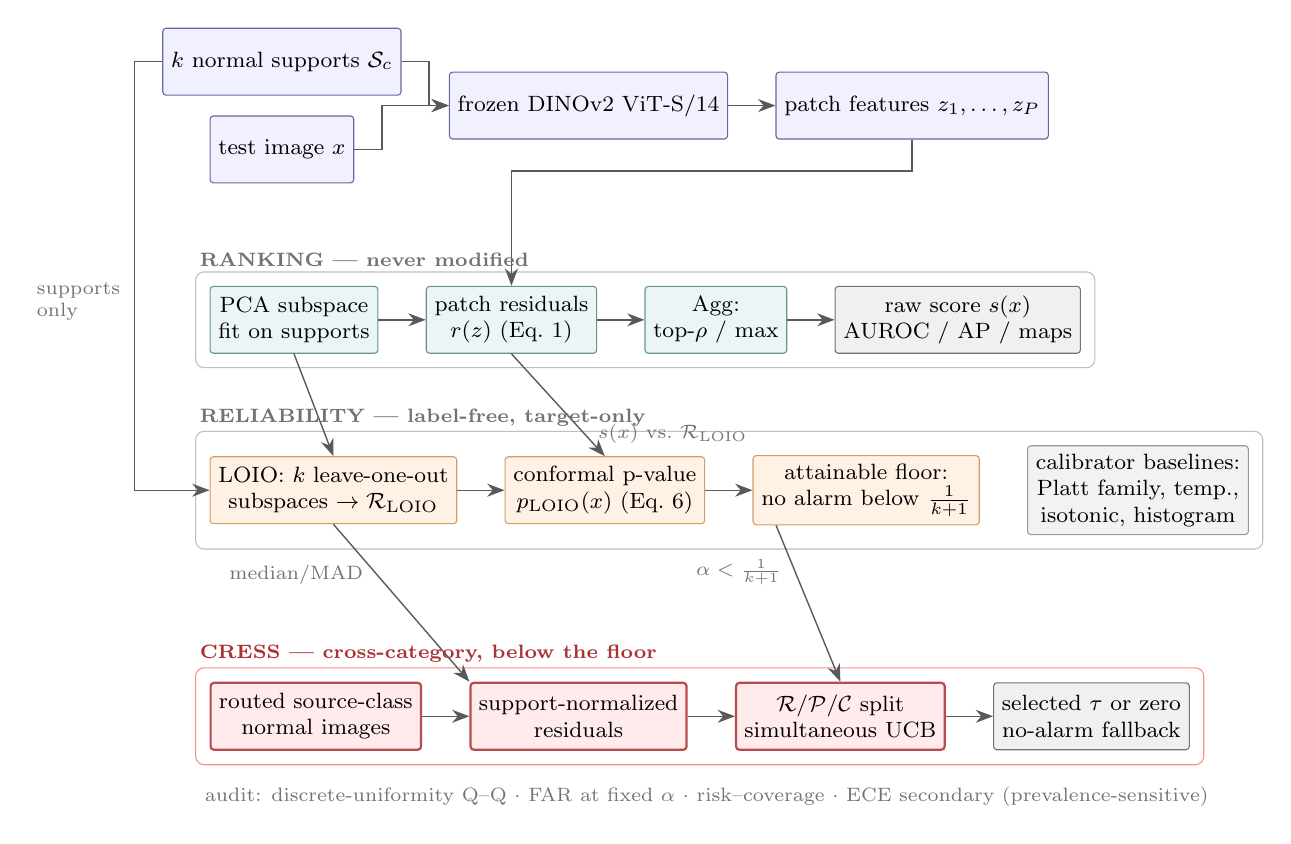
\begin{tikzpicture}[
  font=\footnotesize,
  node distance=4.5mm and 6mm,
  box/.style={draw=black!60, rounded corners=1.2pt, fill=black!4, align=center, inner sep=3pt, minimum height=8.5mm},
  input/.style={box, fill=blue!6, draw=blue!40!black!60},
  rank/.style={box, fill=teal!8, draw=teal!60!black!60},
  rel/.style={box, fill=orange!10, draw=orange!70!black!60},
  sc3r/.style={box, fill=red!8, draw=red!60!black!70, thick},
  outbox/.style={box, fill=black!6, draw=black!55},
  lane/.style={draw=black!25, rounded corners=3pt, inner sep=5pt},
  lanelabel/.style={font=\scriptsize\bfseries, text=black!55, anchor=south west, inner sep=1.5pt},
  arr/.style={-{Stealth[length=2.2mm]}, black!65, line width=0.5pt},
  note/.style={font=\scriptsize, text=black!55, align=center},
]

% ---------------- row 1: shared trunk ----------------
\node[input] (support) {$k$ normal supports $\mathcal{S}_c$};
\node[input, below=2.5mm of support] (test) {test image $x$};
\node[input, right=9mm of $(support.east)!0.5!(test.east)$, anchor=west] (backbone) {frozen DINOv2 ViT-S/14};
\node[input, right=of backbone] (feats) {patch features $z_1,\dots,z_P$};
\draw[arr] (support.east) -- ++(3.5mm,0) |- (backbone.west);
\draw[arr] (test.east) -- ++(3.5mm,0) |- (backbone.west);
\draw[arr] (backbone) -- (feats);

% ---------------- row 2: ranking lane ----------------
\node[rank, below=13mm of test.south west, anchor=north west] (pca) {PCA subspace\\fit on supports};
\node[rank, right=of pca] (resid) {patch residuals\\$r(z)$ (Eq.~1)};
\node[rank, right=of resid] (agg) {$\operatorname{Agg}$:\\top-$\rho$ / max};
\node[outbox, right=of agg] (rankout) {raw score $s(x)$\\AUROC / AP / maps};
\draw[arr] (pca) -- (resid);
\draw[arr] (resid) -- (agg);
\draw[arr] (agg) -- (rankout);

% ---------------- row 3: reliability lane ----------------
\node[rel, below=13mm of pca.south west, anchor=north west] (loio) {LOIO: $k$ leave-one-out\\subspaces $\to \mathcal{R}_{\mathrm{LOIO}}$};
\node[rel, right=of loio] (pval) {conformal p-value\\$p_{\mathrm{LOIO}}(x)$ (Eq.~6)};
\node[rel, right=of pval] (floor) {attainable floor:\\no alarm below $\tfrac{1}{k+1}$};
\node[box, right=of floor, fill=black!5, draw=black!40] (calib) {calibrator baselines:\\Platt family, temp.,\\isotonic, histogram};
\draw[arr] (loio) -- (pval);
\draw[arr] (pval) -- (floor);

% ---------------- row 4: CRESS ----------------
\node[sc3r, below=20mm of loio.south west, anchor=north west] (sc3rsrc) {routed source-class\\normal images};
\node[sc3r, right=of sc3rsrc] (sc3rnorm) {support-normalized\\residuals};
\node[sc3r, right=of sc3rnorm] (sc3rthr) {$\mathcal R/\mathcal P/\mathcal C$ split\\simultaneous UCB};
\node[outbox, right=of sc3rthr] (alarmout) {selected $\tau$ or zero\\no-alarm fallback};
\draw[arr] (sc3rsrc) -- (sc3rnorm);
\draw[arr] (sc3rnorm) -- (sc3rthr);
\draw[arr] (sc3rthr) -- (alarmout);

% ---------------- inter-lane arrows ----------------
\draw[arr] (feats.south) -- ++(0,-4mm) -| (resid.north);
\draw[arr] (support.west) -- ++(-3.5mm,0) |- node[note, left, pos=0.28, align=left, xshift=-0.6mm]{supports\\only} (loio.west);
\draw[arr] (pca.south) -- (loio.north);
\draw[arr] (resid.south) -- node[note, right, pos=0.78, xshift=0.5mm]{$s(x)$ vs.\ $\mathcal{R}_{\mathrm{LOIO}}$} (pval.north);
\draw[arr] (loio.south) -- node[note, left, pos=0.32, xshift=-0.5mm]{median/MAD} (sc3rnorm.north west);
\draw[arr] ($(floor.south west)+(3mm,0)$) -- node[note, left, pos=0.3, xshift=-0.5mm]{$\alpha<\tfrac{1}{k+1}$} (sc3rthr.north);

% ---------------- lane frames ----------------
\begin{scope}[on background layer]
\node[lane, fit=(pca)(rankout)] (rankframe) {};
\node[lane, fit=(loio)(floor)(calib)] (relframe) {};
\node[lane, fit=(sc3rsrc)(alarmout), draw=red!45] (sc3rframe) {};
\end{scope}
\node[lanelabel] at (rankframe.north west) {RANKING --- never modified};
\node[lanelabel] at (relframe.north west) {RELIABILITY --- label-free, target-only};
\node[lanelabel, text=red!60!black!80] at (sc3rframe.north west) {CRESS --- cross-category, below the floor};

% ---------------- diagnostics strip ----------------
\node[note, anchor=north west, yshift=-1.5mm] at (sc3rframe.south west)
  {audit: discrete-uniformity Q--Q $\cdot$ FAR at fixed $\alpha$ $\cdot$ risk--coverage $\cdot$ ECE secondary (prevalence-sensitive)};

\end{tikzpicture}
\end{document}
